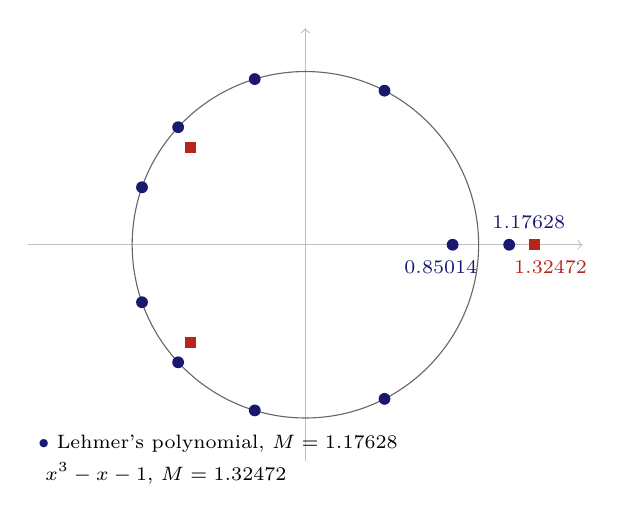
\begin{tikzpicture}[font=\scriptsize]
\draw[black!25,->] (-3.52,0) -- (3.52,0); \draw[black!25,->] (0,-2.75) -- (0,2.75);
\draw[black!60] (0,0) circle (2.200);
\fill[MidnightBlue] (2.588,0.000) circle (0.075);
\fill[MidnightBlue] (1.870,0.000) circle (0.075);
\fill[MidnightBlue] (1.005,1.957) circle (0.075);
\fill[MidnightBlue] (1.005,-1.957) circle (0.075);
\fill[MidnightBlue] (-0.643,2.104) circle (0.075);
\fill[MidnightBlue] (-0.643,-2.104) circle (0.075);
\fill[MidnightBlue] (-1.616,1.493) circle (0.075);
\fill[MidnightBlue] (-1.616,-1.493) circle (0.075);
\fill[MidnightBlue] (-2.075,0.730) circle (0.075);
\fill[MidnightBlue] (-2.075,-0.730) circle (0.075);
\fill[BrickRed] (2.914,0.000) +(-0.07,-0.07) rectangle +(0.07,0.07);
\fill[BrickRed] (-1.457,1.237) +(-0.07,-0.07) rectangle +(0.07,0.07);
\fill[BrickRed] (-1.457,-1.237) +(-0.07,-0.07) rectangle +(0.07,0.07);
\node[above,MidnightBlue] at (2.838,0.08) {$1.17628$};
\node[below,MidnightBlue] at (1.720,-0.08) {$0.85014$};
\node[below,BrickRed] at (3.114,-0.08) {$1.32472$};
\node[right] at (-3.520,-2.530) {\textcolor{MidnightBlue}{$\bullet$} Lehmer's polynomial, $M=1.17628$};
\node[right] at (-3.520,-2.904) {\textcolor{BrickRed}{$\blacksquare$} $x^3-x-1$, $M=1.32472$};
\end{tikzpicture}
